% !TeX root = main.tex
\section{Methodology} \label{sec:method}

In this section, we provide a detailed overview of the context in which our study was conducted, including the setting, participant details, measurement tools employed, and the research methodology adopted.

\subsection{Setting and Participants}
The research was conducted within an Artificial Intelligence (AI) elective course, consisting of three credits. In our institute, three credits correspond to a total of nine hours of work during a week, including three 1 hour lectures. This occurred during the Fall semester of 2023 at a large private university in India. The study involved 105 junior and senior undergraduate students pursuing computer science and information systems degrees. Among the participants, 98 were male, and 7 were female, all within the age range of 18 to 21 and hailing from India. The course employed a continuous evaluation method, with 30\% allocated to two programming assignments, 30\% to a mid-term closed-book examination, and 40\% to a comprehensive closed-book final examination at the end of the term.

\subsection{Measures}
The following measures were used in the study:
\subsubsection{The International Personality Item Pool (IPIP)}
The International Personality Item Pool (IPIP)\footnote{\url{https://ipip.ori.org/}} stands as a comprehensive resource for personality assessment items, facilitating research in psychology across diverse cultural settings. Established in the 1990s by Goldberg \cite{Goldberg}, the IPIP offers an extensive array of self-report measures to assess various dimensions of personality, including the Big Five traits: openness, conscientiousness, extraversion, agreeableness, and neuroticism. In this study, participants' Big Five personality traits were evaluated using the rigorous and comprehensive 120-item version of the IPIP \cite{JOHNSON201478}. This choice was made because the 120-item version strikes a balance, being neither too brief (like the 50-item version) nor overly extensive (like the 300-item version), thus enabling completion within a reasonable timeframe of less than 30 minutes, which is suitable for students.

The 120-item version of the IPIP scale comprises 24 items for each subscale, totaling 120 items. Participants assess the degree to which each item (question or statement) reflects their personality on a 5-point Likert scale, ranging from 1 = very inaccurate to 5 = very accurate. The internal consistency coefficients (Cronbach's alpha) for the five subscales ranged from \begin{math} \alpha \end{math} = 0.84 to 0.93, with values for extraversion at 0.92, agreeableness at 0.85, conscientiousness at 0.84, neuroticism at 0.90, and openness to experience at 0.93. These coefficients signify the reliability of the scale in measuring each personality trait, with higher values indicating greater internal consistency among the items within each subscale.

\subsubsection{Plagiarism Detection}

The Measure of Software Similarity (MOSS) tool \cite{MOSS} was used to detect plagiarism in the programming assignments through collusion among students. MOSS provided a percentage-based measure of similarity between code submissions, allowing for the quantification of plagiarism in each of the two programming assignments. The following command was used to get the count of similar lines: 
\begin{verbatim}
./moss.pl -l python -b ProgramBaseFile/Base_program.py \
Programs/*.py
\end{verbatim}

MOSS usually reports all code matches in pairs of program files. However, when a `base file' is provided using the \textbf{-b} option, the lines of code present in the base file are not counted in the matches reported by MOSS. This ensures that any matching code between two students is not due to the base program provided by the instructor for the programming assignment. The preference for the MOSS tool over JPlag or other source code plagiarism detection tools stemmed from the authors' familiarity with MOSS. In future studies, we intend to incorporate multiple tools to ensure comprehensive plagiarism detection, acknowledging the limitations of relying solely on one tool.

\subsection{Research Design}

As depicted in Figure \ref{fig:activityTimeline}, the first programming assignment was given two weeks from the start of the semester. The second programming assignment was given ten weeks from the start of the semester. Owing to the significant usage of honor pledges to educate students on academic integrity expectations in literature (as discussed in Sec \ref{sec:relatedwork}), we asked students to take an honor pledge during the ninth week. The honour pledge was a pre-requisite for the second programming assignment, all the students 105 students participated in the pledge. 

The Big Five personality trait assessment test was done after the students submitted the second programming assignment during the twelfth week. This sequencing was deliberate to prevent students from discerning our interest in studying their behavior during the programming assignment. The first programming assignment was rolled out without explicit guidance or instructions regarding plagiarism. (However, it was mentioned in the course handout that plagiarism in programming assignments will be strictly dealt with as per the institute policy.)

\begin{figure}[H]
  \centering
  \frame{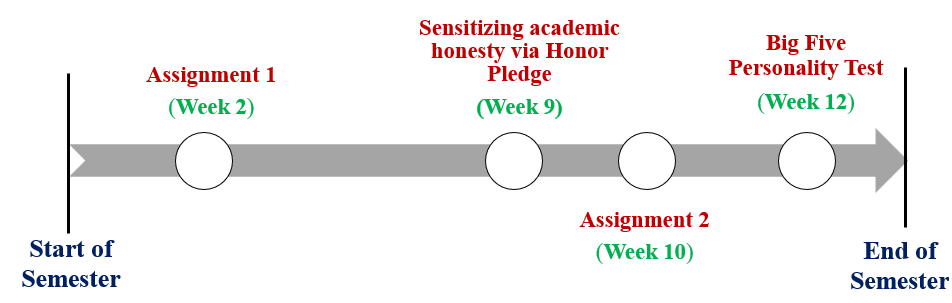
\includegraphics[width=\columnwidth]{SeriesOfactivities.png}}\vspace{-8pt}
  \caption{Series of activities}
  \label{fig:activityTimeline} \vspace{-10pt}
\end{figure}

 The data on personality traits and plagiarism scores, obtained through the Measure of Software Similarity (MOSS) for assignment 1, were utilized to address research question RQ\ref{RQ1}.

In the ninth week, all students had to read and endorse an honor/integrity pledge concerning plagiarism and collusion. This was aimed at raising awareness about plagiarism and upholding academic integrity. It explicitly outlined the behaviors considered plagiarism and collusion. The pledge was administered via a Google form, and a digital signature was mandated from each participant, signifying their commitment to refraining from plagiarism and collusion. Instead of in-class instruction, we opted for this method to ensure that all participants had sufficient time to comprehend the concepts of plagiarism and collusion without sacrificing any class time. The pledge remained accessible for a week and was mandatory. An excerpt from the honor pledge is provided below:

\begin{myquote}
    \textit{The assignments are to be done individually by each student. The objective of the assignments is to help students deepen their understanding of some of the concepts in AI. A secondary objective of the assignments is to help students get better at Python programming.}
    \textbf{Each} of the following amounts to violations of academic integrity:
    \begin{itemize}
        \item \textit{Sharing a part or whole of your program with another student even if one of the students changes the variable names and function names and rearranges the functions within the program file.}
        \item \textit{Sharing a part or whole of your report with another student even if one of the students changes most of the sentences so that superficially, the reports look different. You must cite the resources you have referred in the report.} 
        \item \textit{Getting parts of your program from past programming assignment submissions or internet sources. Each student must do the assignment individually.}
        \item \textit{Sharing code for commonly needed functionality by calling it "driver program" amounts to a violation of academic integrity because one of the objectives of this assignment is to help students get better at Python programming. }
    \end{itemize}
\end{myquote}
The second assignment served as the post-intervention assessment, allowing for the evaluation of the impact of plagiarism awareness on participant behavior.

Both programming assignments were original and did not have pre-existing solutions available on the internet. Below, we provide a brief overview of each assignment for the reader's understanding:

\subsubsection{First Programming Assignment:} The assignment centered on multi-armed bandit concepts and the Markov reward process. Students were tasked to develop a driver program that applied the concepts learned in class. Specifically, they were required to create a Python program capable of adjusting parameters within a provided AI model and visually representing the alterations on a graph. Additionally, students had to report all the findings along with the conclusion and rationale (as comments in the code). All relevant parameters and anticipated outcomes were covered in class, with the professor and teaching assistants available for any inquiries, during the designated assignment period via office hours. The following are the assignment's learning outcomes (LO) with their corresponding Revised Bloom Taxonomy \cite{bloomsTaxonomy} verbs in bold:
\begin{itemize}
    \item \textbf{Understand and Apply} multi-armed bandit and Markov reward process concepts. 
    \item \textbf{Analyze} parameter manipulation and visualization techniques. 
    \item \textbf{Implement} python programs efficiently 
\end{itemize}

\subsubsection{Second Programming Assignment:} The second assignment was based on the game `Connect 4'\footnote{\url{https://en.wikipedia.org/wiki/Connect_Four}}. Specifically, students were given the stub code for one version of the game that they could play and were tasked with modifying and enhancing the given program incrementally that plays against a Myopic player (a player that only views a fixed number of possibilities to evaluate a game state and not all possibilities) using the game tree-based search techniques and constraints given. Also, the students were given clear guidelines and steps to incrementally improve their player function by techniques like `Alpha-Beta Pruning'. The following are the assignment's LO's:
\begin{itemize}
    \item \textbf{Apply} game tree-based techniques and alpha-beta pruning effectively.
    \item \textbf{Implement} an incremental solution with retrospection after each stage.  
    \item \textbf{Comprehend} given python program and enhance it.
\end{itemize}

\subsection{Procedures for data collection and analysis}
\subsubsection{Personality Traits Data:} Following the institute's Human Ethical Committee (HEC) policy, participants were required to provide informed consent before participating in the study. Upon obtaining consent, participants underwent the International Personality Item Pool (IPIP) personality test, which assesses the Big Five personality traits. The test was administered through an online tool available at the provided URL\footnote{\url{https://bigfive-test.com/}}.

After completing the test, participants' final scores for each Big Five personality trait were recorded in a Google form after obtaining the informed consent form as approved by the HEC. To ensure confidentiality and protect participants' privacy, all data collected was anonymized, meaning any personally identifiable information was removed or obscured.

\subsubsection{Assignment Data:} 
Both assignments were administered using Moodle, the institute's learning management system. Upon completion, the source codes for both assignments were subjected to analysis using the Measure of Software Similarity (MOSS) tool to generate plagiarism reports.

To ensure confidentiality, the data was anonymized before processing. The plagiarism scores corresponding to each student (either via collusion or direct plagiarism from other sources), derived from the MOSS reports, were then stored in cloud storage for subsequent analysis. The plagiarism score for each student was calculated based on the proportion of code similarity detected by MOSS. Specifically, it was determined by dividing the maximum number of lines copied from other sources by the total number of lines in the student's source code (ignoring the empty lines). This approach provided a quantitative measure of the extent of plagiarism in each student's assignment.